\documentclass[a4paper,12pt]{article}

\usepackage[spanish]{babel}
\usepackage[utf8]{inputenc}
\usepackage[T1]{fontenc}
\usepackage[utf8]{inputenc}
\usepackage{makeidx}
\usepackage{graphicx}
\usepackage{lmodern}
\usepackage{kpfonts}
\usepackage[left=2cm,right=2cm,top=2cm,bottom=2cm]{geometry}
\usepackage{amsmath,amsfonts,amssymb}
\usepackage{hyperref}
\hypersetup{
    colorlinks=true,
    linkcolor=cyan,
    filecolor=magenta,      
    urlcolor=blue,
    pdftitle={titulo},
    pdfpagemode=FullScreen,
    }
\urlstyle{same}
\usepackage{wrapfig}
\usepackage[rightcaption]{sidecap}


\title{Asignación 2}

\begin{document}

\begin{center}
\par 
\includegraphics[scale=1]{USB} \par
Universidad Simon Bolivar \\ Curso: CI4325 / Interfaces con el Usuario \\ Trimestre: Enero-Marzo, 2024 \\ Profesor: Franco Gabriel Nori Gonzalez \\ Estudiante: Junior Miguel Lara Torres - Carnet: 17-10303 \\
\end{center}

\begin{center}
Asignación 2 (5\%)
\end{center}

	Haciendo uso de los conceptos vistos en las clase de “principios de diseño” se desea que usted realice de manera individual la siguinete actividad:

\begin{itemize}
\item Vea el siguiente video: \url{https://www.youtube.com/watch?v=Wac3aGn5twc}.
\item Encuentre en el mismo elementos visuales, interactivos y psicológicos que estén fallando en el diseño presentado durante el proceso y respecto al producto final.

\item Deberá hallar al menos 5 elementos para que su evaluación se considere completa.
\end{itemize}

	A continuación se muestra por etapas la transformación del logo incial de STOP segun el video. \\

\begin{SCfigure}[0.8][h]
\caption{Se observa como en esta primera etapa se pierde \textbf{Unidad} al agregar logos de socios adicionales, inclusión de texto, colores y flechas con texto que nada que ver con el propósito del producto. A pesar de que existe variedad de colores estos no tienen los tonos adecuados en pro de conseguir contrastes notorios que permiten la correcta lectura y comunicación del mensaje que es "PARE". Tambíén se observa que la \textbf{Economía de los Elementos} empieza a fallar dado que existen varios elementos distractores.}
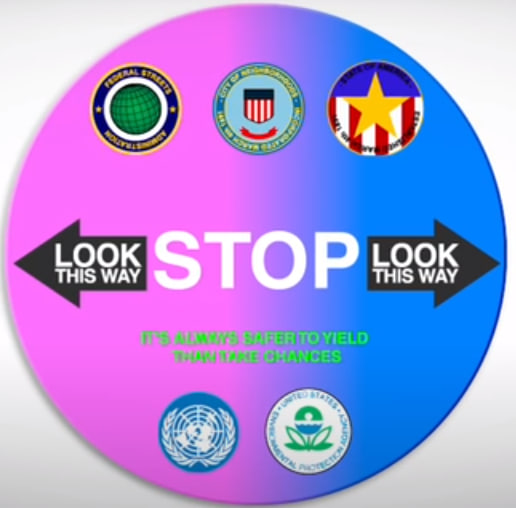
\includegraphics[width=0.5\textwidth]{logop1}
\end{SCfigure}

\begin{SCfigure}[0.8][h]
\caption{En esta etapa se observa como se pierde, desde el punto de tamaños, el logo de la empresa pasa a tener mayor atracción mientras que el mensaje principal pasa a tener menor, claro esta que la distribución de los elementos no es equitativa(\textbf{Proporción y Balance}). Adicionalmente el trayecto natural que sigue la vista es ambiguo debido a los elementos "Look this way" desconcentrando el verdadero punto de atención(\textbf{Jerarquia y Dominancia}).}

\includegraphics[width=0.5\textwidth]{logop2}
\end{SCfigure}

\begin{SCfigure}[0.8][h]
\caption{La inserciön de imagen de la chica hablando al teléfono con la finalidad de dar a entender "en que ocasión debes detenerte" no parece dar con el aspecto psicológico ideal hacia el mensaje que se quiere transmitir desde un principio (\textbf{Efecto del Diseño Atractivo}).}
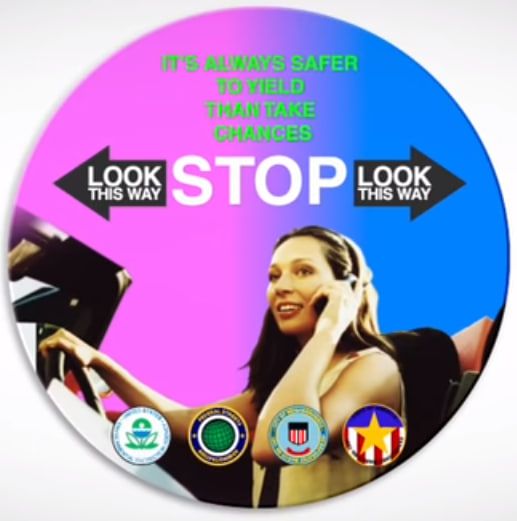
\includegraphics[width=0.5\textwidth]{logop3}
\end{SCfigure}

\begin{SCfigure}[0.8][h]
\caption{Se incluye elementos llamativos y cambio de nombre perdiendo asi el foco principal del mensaje. De esta forma tienen un impacto llamativo pero no al lugar correcto, asi que por más beneficioso que se tenga en un aspecto no necesariamente es lo correcto (\textbf{Efecto del Diseño Atractivo}). Por otro lado, el cambio de circulo a octogonal no favorece en el aspecto psicologico, esto según el criterio teórico de que "la cantidad de lados de los polígonos están relacionados al grado de peligrosidad que supone la intersección", en este caso el circulo tiene infinitos lados lo que supone el nivel más alto de peligrosidad.(\textbf{Diseño Emocional})}
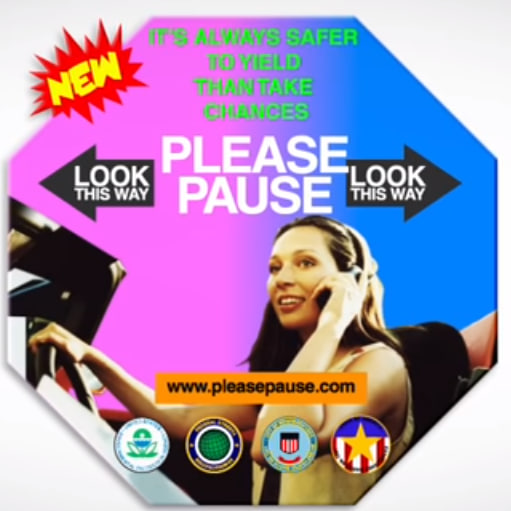
\includegraphics[width=0.5\textwidth]{logop4}
\end{SCfigure}

\begin{SCfigure}[0.8][h]
\caption{Esta etapa final termine de incluir muchos elementos distractores, un cambio completo de mensaje y dificultad de contraste. Se termine llenando de texto que para lo que debe ser una señal de tránsito no tiene sentido debido a la circunstancias en que esta aporta un mensaje(conduciendo). También observamos un force de interacción con el link hacia la página web, donde se supone que la interacción con el usuario no debe ir mas allá de advertencion al peaton/conductor, en este sentido se busca que el usuario genere acciones al tratar de visitar el sitio web(\textbf{Economía del Movimiento}).}
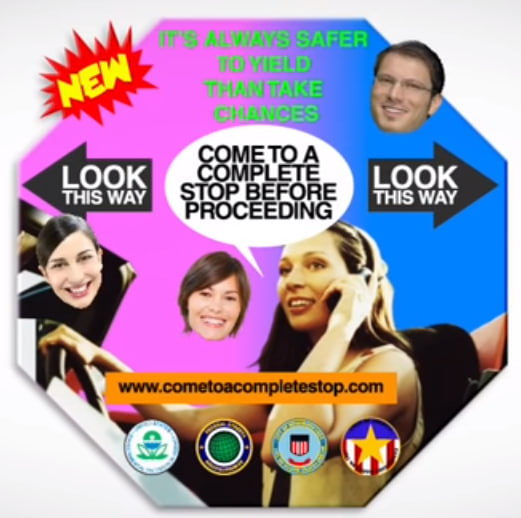
\includegraphics[width=0.5\textwidth]{logop5}
\end{SCfigure}

\end{document}